\chapter{Components of an interactive map}\label{CInteractiveMap}
When creating an interactive map one must consider which features to add to enhance the user experience. To give an overview of some of the basic features used for navigating and get information from a interactive map www.openstreetmap.org has been used as an example. \citep{OpenStreetMap} A picture of this map can be seen in figure \ref{InteractiveMap}. Its User Interfaces (UI) have been numbered with boxes. These boxes have been colored based on how useful the function would be for exploring and comparing large population dataset. The green are essential, the yellow are useful and the red are not relevant. The reasoning behind the coloring is explained in section \ref{SortingFunctions}.


\begin{figure} [H]
	\centering
	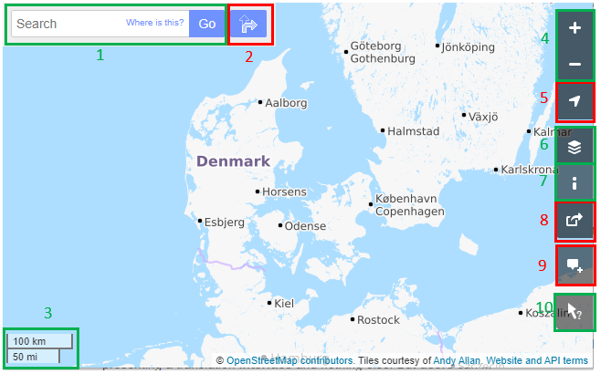
\includegraphics[width=.8\textwidth]{Pictures/InteractiveMap}
	\caption{An example of an interactive map, Openstreetmap. The user interface components have been colored green if it is deemed useful for the developed tool or otherwise red. Source: \citep{OpenStreetMap}}
	\label{InteractiveMap}
\end{figure}



What the different parts of the UI do can be seen in table \ref{tabOSMFunctions}. The functions of the UI can be classified in five different categories. Using the map navigation UI the user can control which part of the map is being displayed.
The real-life navigation tool is used for navigating in the real world. 
The map explanation category gives the user information about the map. This can be general information about the scale or symbols on the map or specific information about a clicked point. 
The tool for controlling the displayed data is used for controlling what is being visualized on the map. The last category, communication with others, is for sharing information with other users of the map. 

\begin{table}[h]
	\centering
	\begin{tabular}{l}
		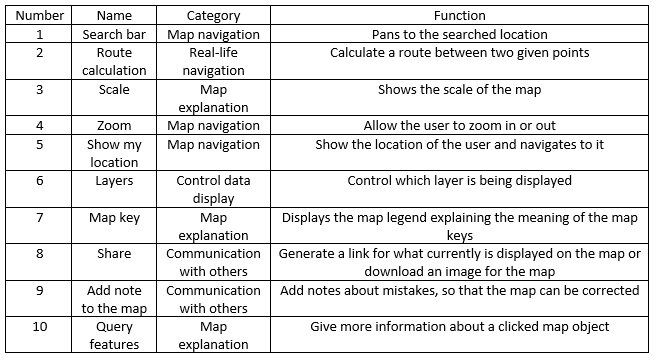
\includegraphics[width=0.8\textwidth]{Pictures/tabOSMFunctions}
	\end{tabular}
	\caption{Overview of the UI elements highlighted in figure \ref{InteractiveMap}}
	\label{tabOSMFunctions}
\end{table}

\section{Relevant functionalities}\label{SortingFunctions}

The essential functionalities are the searchbar, zooming and Map key. 
Having a search bar allows the user to quickly pan to an area of interest and the zoom function allows the user to control the extent. Having a legend is also central to explain to the user which values the colors of the raster would correspond to. 


The useful functions are the scale, the layer control, parts of the share function and the Query features. A scale can help the user get a sense of scale. However, this is only useful if the scale is presented with a unit, which the user easily can comprehend. As mentioned in section \ref{caseDataTech} the unit of the projection is in degrees, which would result in the scale also being in degrees. The layer control is important, since this would allow the map to be able to display multiple different population projections. The tool have been developed for single individuals, so the communicating with other is outside of the scope of this project. However it could still be relevant for a single user to be able to save an extent or export an image of the map. Getting more information about a clicked point could also be a beneficial feature. This information could for instance be the exact value in the clicked point. 

The functions which are irrelevant are the route calculation, "Show my location" and "Add note to the map". The first is only useful for route planning, which is not the purpose of this map. The "Show my location" function is not relevant for this target audience. It would be relevant if the target audience was citizens, who just wanted to explore a population projection out of curiosity. These would potentially be interested in knowing what the expected population would be in their neighbourhood. The last function rely on multiple users, which is outside the scope of this project.

\section{Comparing layers}

The functions presented so far does not enable an easy visual comparison of raster data. It is possible currently by changing back and forth between different layers with different population projections. This however is a bit inconvenient. 
An alternative way would be to use comparison layers in a similar fashion to how it currently is being done with the makeCityWebsite tool mentioned in section \ref{MakeCitySection}. This would require the creation of comparison layers for each combination of SSPs and years, which should be compared.   
A third option would be to display multiple maps at the same time as illustrated in figure \ref{DualMapExample}. These two maps are linked together by a shared view. The means the panning or zooming in one map would do the same operation on the other map.

\begin{figure} [H]
	\centering
	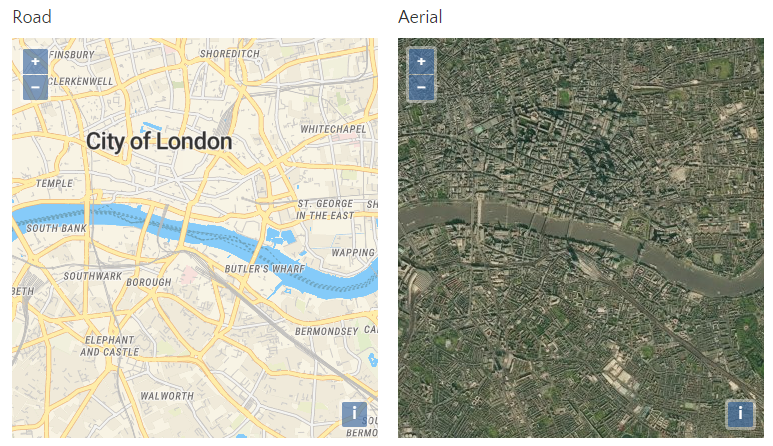
\includegraphics[width=.8\textwidth]{Pictures/DualMapExample}
	\caption{An example of two maps sharing the same view. Source: \citet{DualmapExample}}
	\label{DualMapExample}
\end{figure}


This third option was chosen.